% LAB 3:
% Modeling and Simulation Case Studies

\Opensolutionfile{ModSimSolutions}
% \begin{solmodsim}
% \end{solmodsim}

\chapter{Modeling and Digital Simulation Case Studies} \label{ch.ModSim}

One of the objectives of this session is to get you acquainted with the basics of Simulink, a graphical modeling, simulation, and prototyping environment used extensively in industry.  We will not be able to cover the vast capability of Simulink with a few examples; you are encouraged to explore various features and graphical programming techniques on your own.
\par
The other objectives of this lab are to find the mathematical model for some basic physical systems, to obtain a digital simulation diagram for the resulting differential equations, and to obtain the system's step response and investigate the effect of damping on the system response.

\section{Pre-Lab Reading}
Read the following introductory material.  More help can be found in Appendix~\ref{app.statespace}.
\par
The dynamic performance of physical systems is obtained by utilizing the related physical laws governing them.  Many dynamic systems contain energy storage elements such as masses and springs (in mechanical systems) or inductors and capacitors (in an electric circuit).  The principle of conservation of energy prohibits instantaneous changes in the state variables. Therefore, the system will go through some transients before settling to their steady-state values.
\par
All physical systems are nonlinear to some extent.  In order to model the system with linear time-invariant differential equations (for transfer function or state space representations), the system must first be linearized.  Alternatively, its range of operation may be confined to a linear range.
\par
The next step in designing a practical control system is to simulate the model on a computer to obtain the system response to various signals and disturbances.  Then we can introduce appropriate controllers to achieve the desired system response.  This process of design and analysis is repeated until a satisfactory control system is obtained and then the design may be implemented on the hardware.
\par
One of the most powerful tools for modeling and simulation of dynamic systems is Simulink, a toolbox extension of MATLAB.  Simulink's strongest selling point is that it is very visual and intuitive.  A system in block diagram representation is built easily and the simulation results are displayed quickly.  Simulation algorithms and parameters can be changed in the middle of a simulation with natural results, thus providing the student with a readily accessible learning tool for simulating many of the operational problems found in the real world.
\par
Simulink is particularly useful for studying the effects of nonlinearities on the behavior of the a system.  As such, it is also an ideal research tool.  Simulink has many advanced features for simulating a complex control system, such as the creation of new subsystem blocks and \uline{masking blocks} through m-files, C programs, or other Simulink models for easy integration in your system's model.  This allows an extension of the Simulink graphical functions to suit your own needs of analysis and design.  The Simulink demos and User's Guide are very helpful in explaining the advanced usage and extension of the Simulink block library.  For more information on Simulink, see Chapter~1 in \cite{saadatbook} or browse \cite{saadatsite}.

\section{Laboratory Procedure}

\begin{casestudy}{Mechanical Translational System} \label{cs.mechtrans}
Consider a simple mechanical system consisting of a mass, spring, and shock absorber---known as a \textit{dashpot} or \textit{piston}---shown in Figure~\ref{fig.mechdiagram}.  In the figure, $M$ is the mass, $B$ is the damping coefficient, $k$ is the spring constant, $f(t)$ is the external force, and $x(t)$ is the displacement of the mass.  Three forces (and inertia) influence the motion of the mass, namely the applied force, the damping force, and the spring force as shown in the free-body diagram in Figure~\ref{fig.freebody}.

\newsavebox{\tempbigA}
\newsavebox{\tempsmallA}
\begin{figure}[bht]
    \centering
    \sbox{\tempbigA}{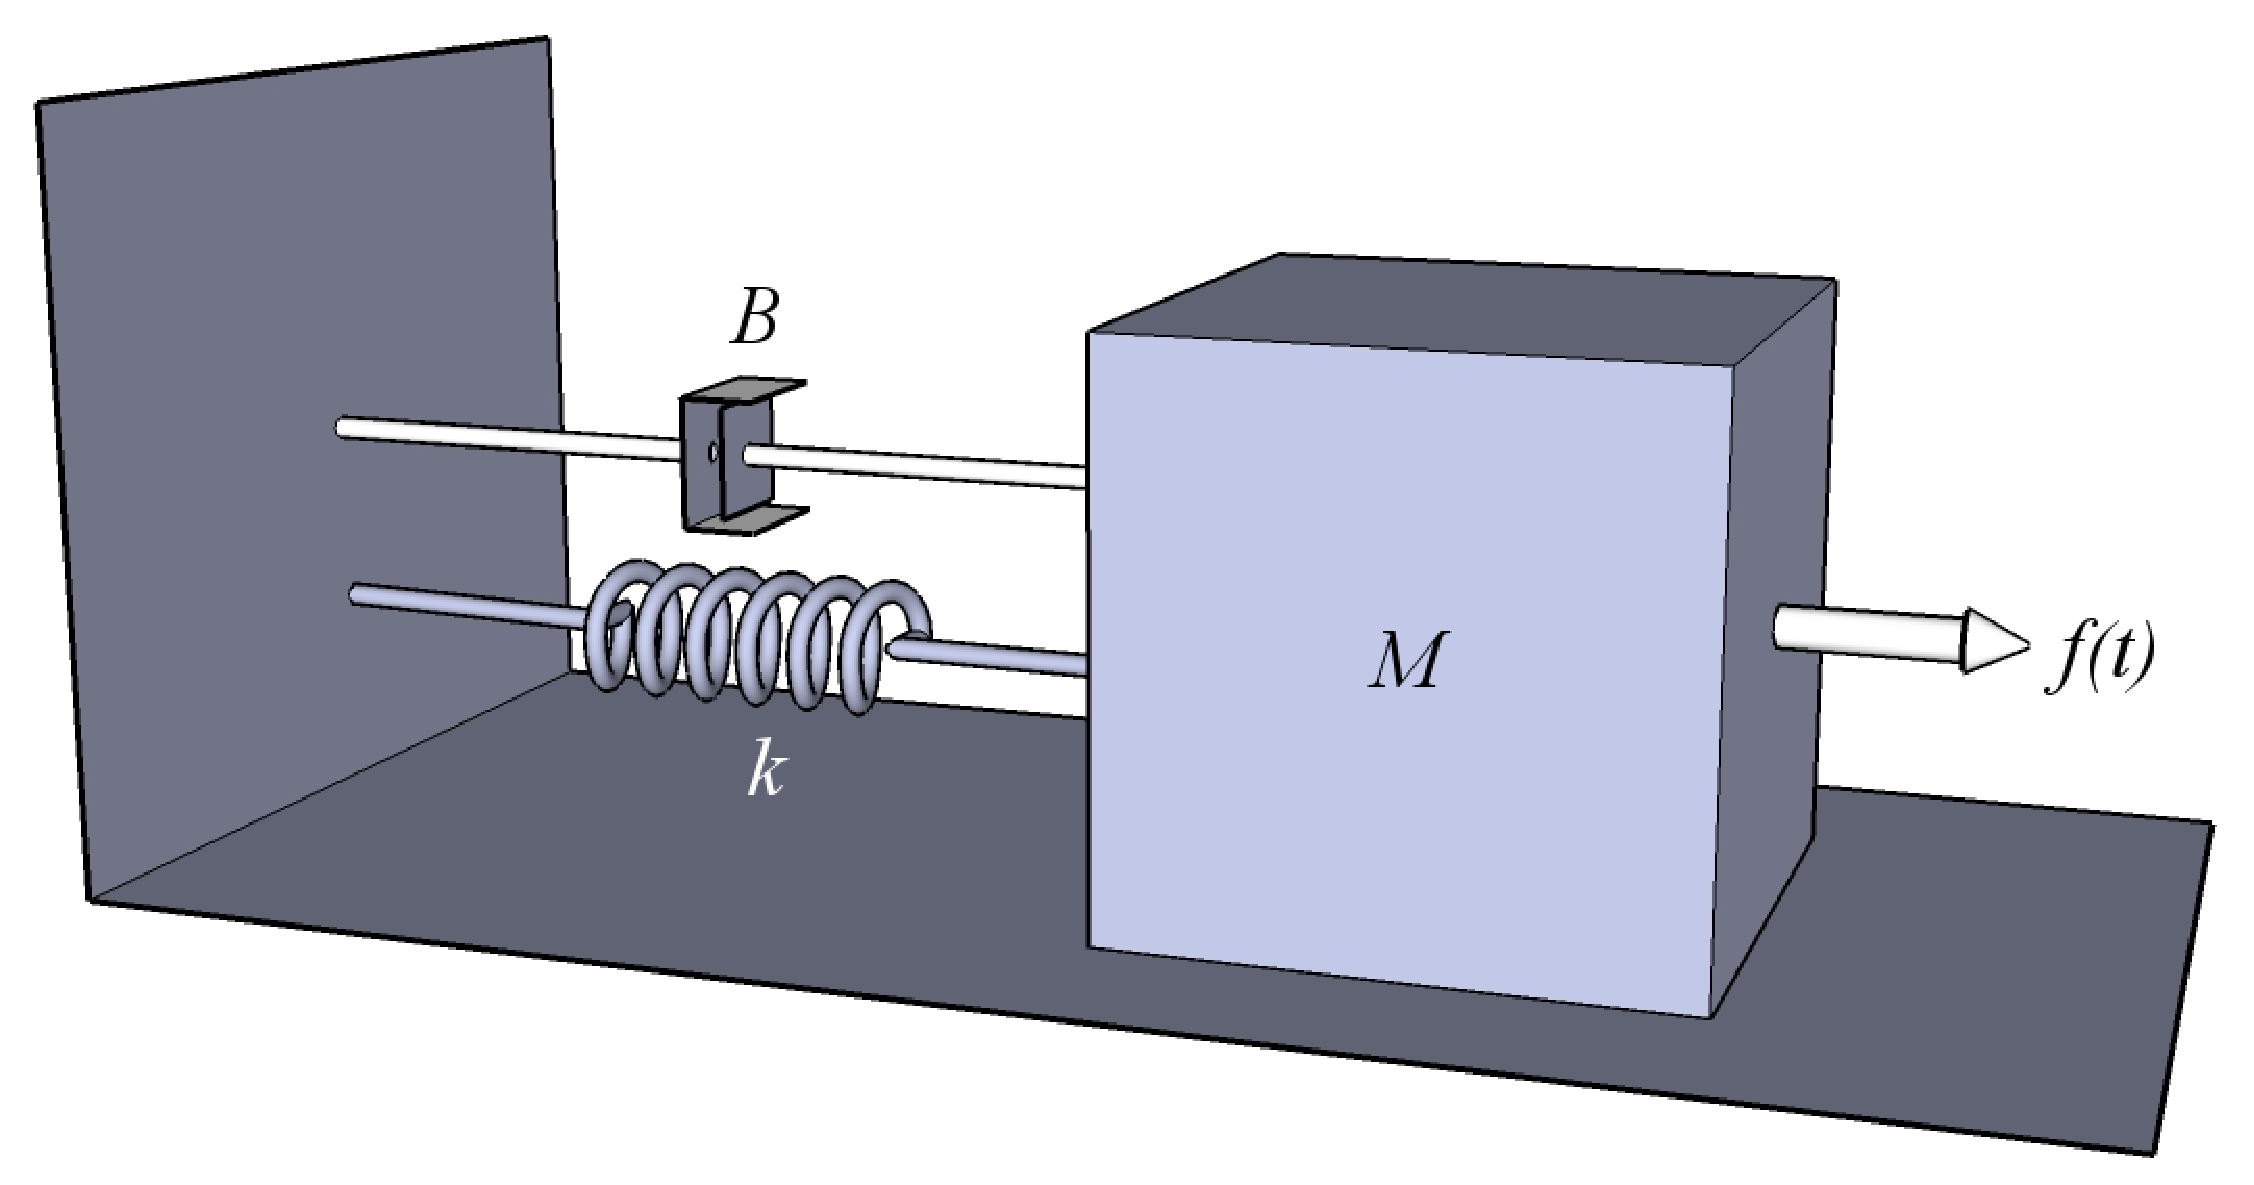
\includegraphics[width=.6\textwidth]{mechdiagram}}
    \sbox{\tempsmallA}{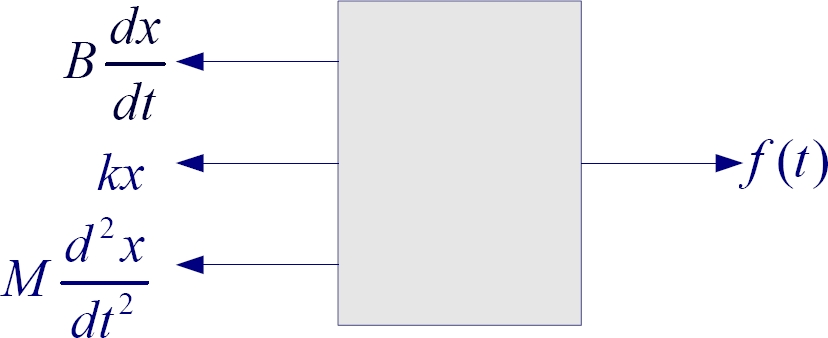
\includegraphics[width=.35\textwidth]{mechfreebody}}
    \newlength{\subfigoffsetA}
    \setlength{\subfigoffsetA}{0.5\ht\tempbigA}
    \addtolength{\subfigoffsetA}{-0.5\ht\tempsmallA}
    \subfloat[
            Mechanical translational system
            \label{fig.mechdiagram}
            ]{
            \usebox{\tempbigA}
            }
    \hfill
    \subfloat[
            Free-body diagram
            \label{fig.freebody}
            ]{
            \raisebox{\subfigoffsetA}{\usebox{\tempsmallA}}
            }
    \caption{}
\end{figure}

Applying Newton's Second Law, we have 
\begin{equation}
    M\frac{d^2 x(t)}{dt^2} + B\frac{d x(t)}{dt} + kx = f(t)
        \label{eq.mechfreebody}
\end{equation}
The transfer function model is obtained by taking the Laplace transform (with zero initial conditions), which results in:
\begin{equation}
    G(s) = \frac{X(s)}{F(s)} = \frac{1}{Ms^2 + Bs + k}
        \label{eq.mechtf}
\end{equation}
You may note that for complicated mechanical systems, it is easier to draw the electric circuit force-voltage analogy in place of the free-body diagram.  In the force-voltage analogy, mass ($M$) is analogous to inductance, spring compliance ($1/K$) is analogous to capacitance, damping coefficient ($B$) is analogous to resistance, and velocity ($\dot{x}$) is analogous to current.  The key point in drawing the electric circuit analogy is to identify the displacement or velocity of each element and draw the circuit accordingly.  The circuit can be drawn in the s-domain to find the transfer function or in the time domain which is suitable for obtaining the state space model.  The electric circuit analogy for this mechanical system is shown in Figure~\ref{fig.mechelecanalogy}.

\begin{figure}[bht]
\centering
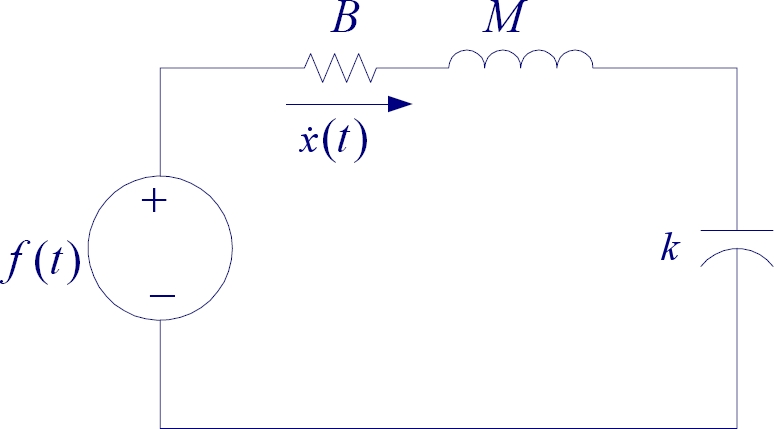
\includegraphics[width=.5\textwidth]{mechelecanalogy}
\caption{\footnotesize
        Electric circuit analogy for the mechanical system in Fig.\ \ref{fig.mechdiagram}
        \label{fig.mechelecanalogy}
        }
\end{figure}

With Kirchhoff's voltage law applied to the electric circuit, we get
\begin{equation}
    M\frac{d\dot{x}(t)}{dt} + B\dot{x}(t) + k\int_0^t \dot{x}(\sigma) = f(t)
\end{equation}
which is of course mathematically equivalent to (\ref{eq.mechfreebody}).  Equation~(\ref{eq.mechfreebody}) can also be written in state space form by selecting the two state variables as displacement and velocity: $x_1(t)=x(t)$ and $x_2(t) = \dot{x}(t)$.  The first-order differential equations then become
\begin{equation} \label{eq.mechdiff}
\begin{split}
    \frac{dx_1(t)}{dt} & = x_2(t) \\
    \frac{dx_2(t)}{dt} & = \frac{1}{M}f(t) - \frac{k}{M}x_1(t) - \frac{B}{M}x_2(t)
\end{split}
\end{equation}
For convenience, we will define multiple outputs: $y_1 = x_1(t)$ and $y_2 = x_2(t)$.  Thus the state space expression of this system is
\begin{equation}
\begin{split}
    \left[ \begin{array}{c} \dot{x}_1(t) \\ \dot{x}_2(t) \end{array} \right]
    & = 
    \left[ \begin{array}{cc} 0 & 1 \\ -\frac{k}{M} & -\frac{B}{M} \end{array}
        \right]
    \left[ \begin{array}{c} x_1(t) \\ x_2(t) \end{array} \right]
    +
    \left[ \begin{array}{c} 0\\ \frac{1}{M} \end{array} \right]
    f(t)
    \\
    \left[ \begin{array}{c} y_1(t) \\ y_2(t) \end{array} \right]
    & =
    \left[ \begin{array}{cc} 1&0\\0&1 \end{array} \right]
    \left[ \begin{array}{c} x_1(t) \\ x_2(t) \end{array} \right]
\end{split}
\end{equation}
The simulation diagram for Equations~(\ref{eq.mechdiff}) is shown in Figure~\ref{fig.mechsimdiagram}

\begin{figure}[bht]
\centering
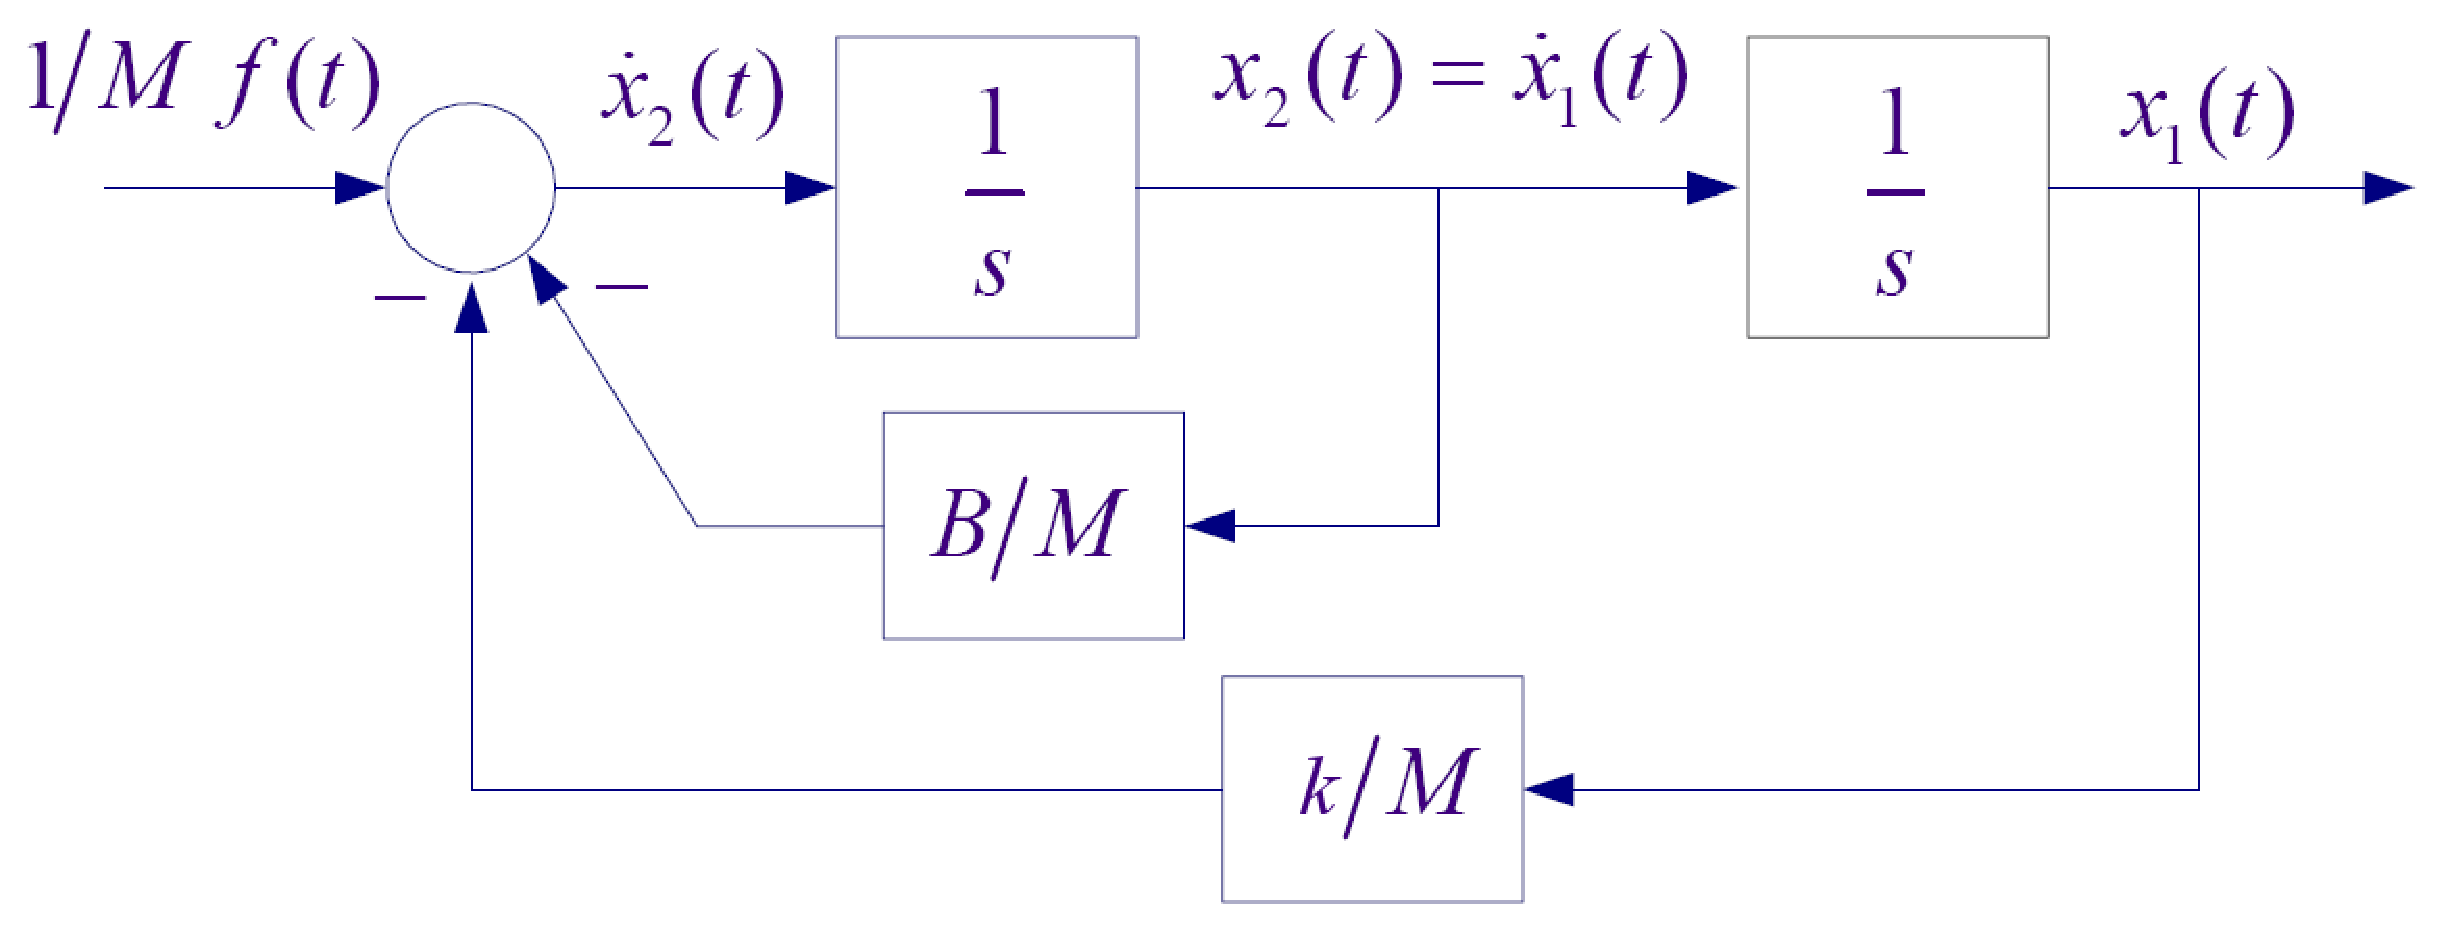
\includegraphics[width=.6\textwidth]{mechsimdiagram}
\caption{\footnotesize
        Simulation diagram for the mechanical system in Case Study~\ref{cs.mechtrans}
        \label{fig.mechsimdiagram}
        }
\end{figure}

With the system initially at rest, a constant force of $f(t) = 32$~Newtons is applied at time $t=0$.  The system in question has a mass of $2$~kg and a spring constant of $32\mbox{ kg}/\mbox{s}^2$.  We are told that the damping coefficient, $B$, may be adjusted to obtain a desirable response.
\par
The system's characteristic equation---from Eq.\ (\ref{eq.mechtf})---is given by
\begin{equation}
    s^2 + \frac{B}{M} s + \frac{k}{M} = 0
\end{equation}
which may be compared to the standard second-order transfer function
\begin{equation}
    s^2 + 2 \zeta \omega_n + \omega_n^2 = 0
\end{equation}

\begin{enumerate}
\item
    \textbf{Perform the following analysis:}
    \begin{enumerate}
    \item
        The dashpot damping is adjusted to $B = 2\mbox{ Ns/m}$.  Determine the natural frequency of oscillation ($\omega_n$), damping ratio ($\zeta$), percent overshoot ($PO = 100e^{-\frac{\zeta\pi}{\sqrt{1-\zeta^2}}}$), peak time ($t_p = \frac{\pi}{\omega_n \sqrt{1-\zeta^2}}$), and settling time ($t_s \approx 4\tau$).
    \item
        jk;asdf
    \end{enumerate}
\item
    ;lakjdf
\end{enumerate}

\end{casestudy}
\begin{casestudy}{
Simple Pendulum}
\label{cs.simplepend}

\end{casestudy}


\begin{thebibliography}{9}
    \bibitem{saadatbook} Hadi Saadat.  Computational Aids in Control Systems Using MATLAB.  McGraw-Hill.  1993.
    \bibitem{saadatsite} Hadi Saadat website. http://people.msoe.edu/~saadat/matlab.htm
\end{thebibliography}

\Closesolutionfile{ModSimSolutions}
